\documentclass[12pt, a4paper]{article}
\usepackage[utf8]{inputenc} 
\usepackage[italian]{babel}
\usepackage{latexsym}
\usepackage{url}
\usepackage{fancyhdr}
\usepackage{graphicx}
\usepackage{amssymb}
\usepackage{multirow}
\title{Calcolo SAD tra due blocchi di immagini}
\author{Carmine Benedetto, Silvio Bianchi}
\date{22 settembre 2011}
%INIZIO INTESTAZIONE
\frenchspacing
\pagestyle{fancy}
\fancyhf{}
\rhead{\bfseries\thepage}
%\renewcommand{\chaptermark}[1]{\markboth{\thechapter.\ #1}{}}
\renewcommand{\sectionmark}[1]{\markboth{\thesection.\ #1}{}}
%FINE INTESTAZIONE
\begin{document}
\maketitle
\newpage
\tableofcontents
\newpage 
\listoffigures
\newpage
\section{Specifiche Formali}
\subsection{Prima fase}
Progettare un circuito digitale sincrono che realizzi il calcolo della \textit{SAD}, definita come
la somma delle differenze in valore assoluto pixel a pixel, tra due blocchi di immagini
monocromatiche A e B. Si considerino blocchi di immagine di dimensioni 16 pixel x 16
pixel, ogni pixel è un numero intero tra 0 e 255 rappresentato su 8 bit. Il circuito ha come
ingressi il segnale di \textit{clock}, un segnale di \textit{reset}, un segnale di \textit{enable} e due segnali \textit{PA} e
 \textit{PB} su cui si ipotizza vengono forniti dall’esterno, in cicli successivi, i 256 pixel dei due
blocchi di immagini A e B. In uscita il circuito ha un segnale \textit{SAD} a 16 bit ed un segnale
\textit{data\_valid} a 1 bit. In condizioni di reset \textit{SAD} = 0 e \textit{Data\_valid} = 0. \textit{Data\_valid} viene settato
alla fine del calcolo della \textit{SAD}. Se \textit{enable} = 0 il circuito conserva il suo stato
indipendentemente dal valore dei segnali di ingresso.
\subsection{Seconda fase}
Terminata la pima fase paramatrizzare la descrizione VHDL estendola al caso generico
di blocchi di dimensione NxN con N potenza di 2.\\
Nota: i segnali di ingresso e di uscita rimangono gli stessi a meno di \textit{SAD} la cui dimensione sarà \textit{n} bit, con $2^n$ $\geq$ (255 * $N^2$ ) ; la temporizzazione viene modificata in quanto vengono ricevuti dall’esterno $N^2$ coppie di pixel.
\newpage
\section{Descrizione dell'algoritmo}
Per realizzare il calcolo della \textit{SAD} che rispettasse le specifiche indicate, è stato progettato, utilizzando il linguaggio di programmazione \textit{VHDL}, un circuito sincrono che ad ogni passo prende in ingresso 1 pixel (rappresentato su 8 bit) per ogni immagine, ne effettua la sottrazione, si ricava poi il valore assoluto del risultato della sottrazione e lo invia ad un buffer che tiene memoria delle precedenti somme. Il calcolo della \textit{SAD} si considera completato (con conseguente settaggio della variabile \textit{data\_valid}) quando sono stati effettuati NxN passi (con NxN numero dei pixel di un'immagine).
\newpage
\section{Architettura selezionata per la realizzazione}
\subsection{Modello architetturale}
Il modello architetturale scelto per la realizzazione dell'applicazione è stato quello di tipo \textit{behavioural}. In seguito viene mostrato il flusso di progettazione relativo al caso specifico con ingressi ad 8 bit ed uscite a 16 bit. Naruralmente il modello è facilmente estendibile al caso generale.
\begin{figure}[h!]
\centering
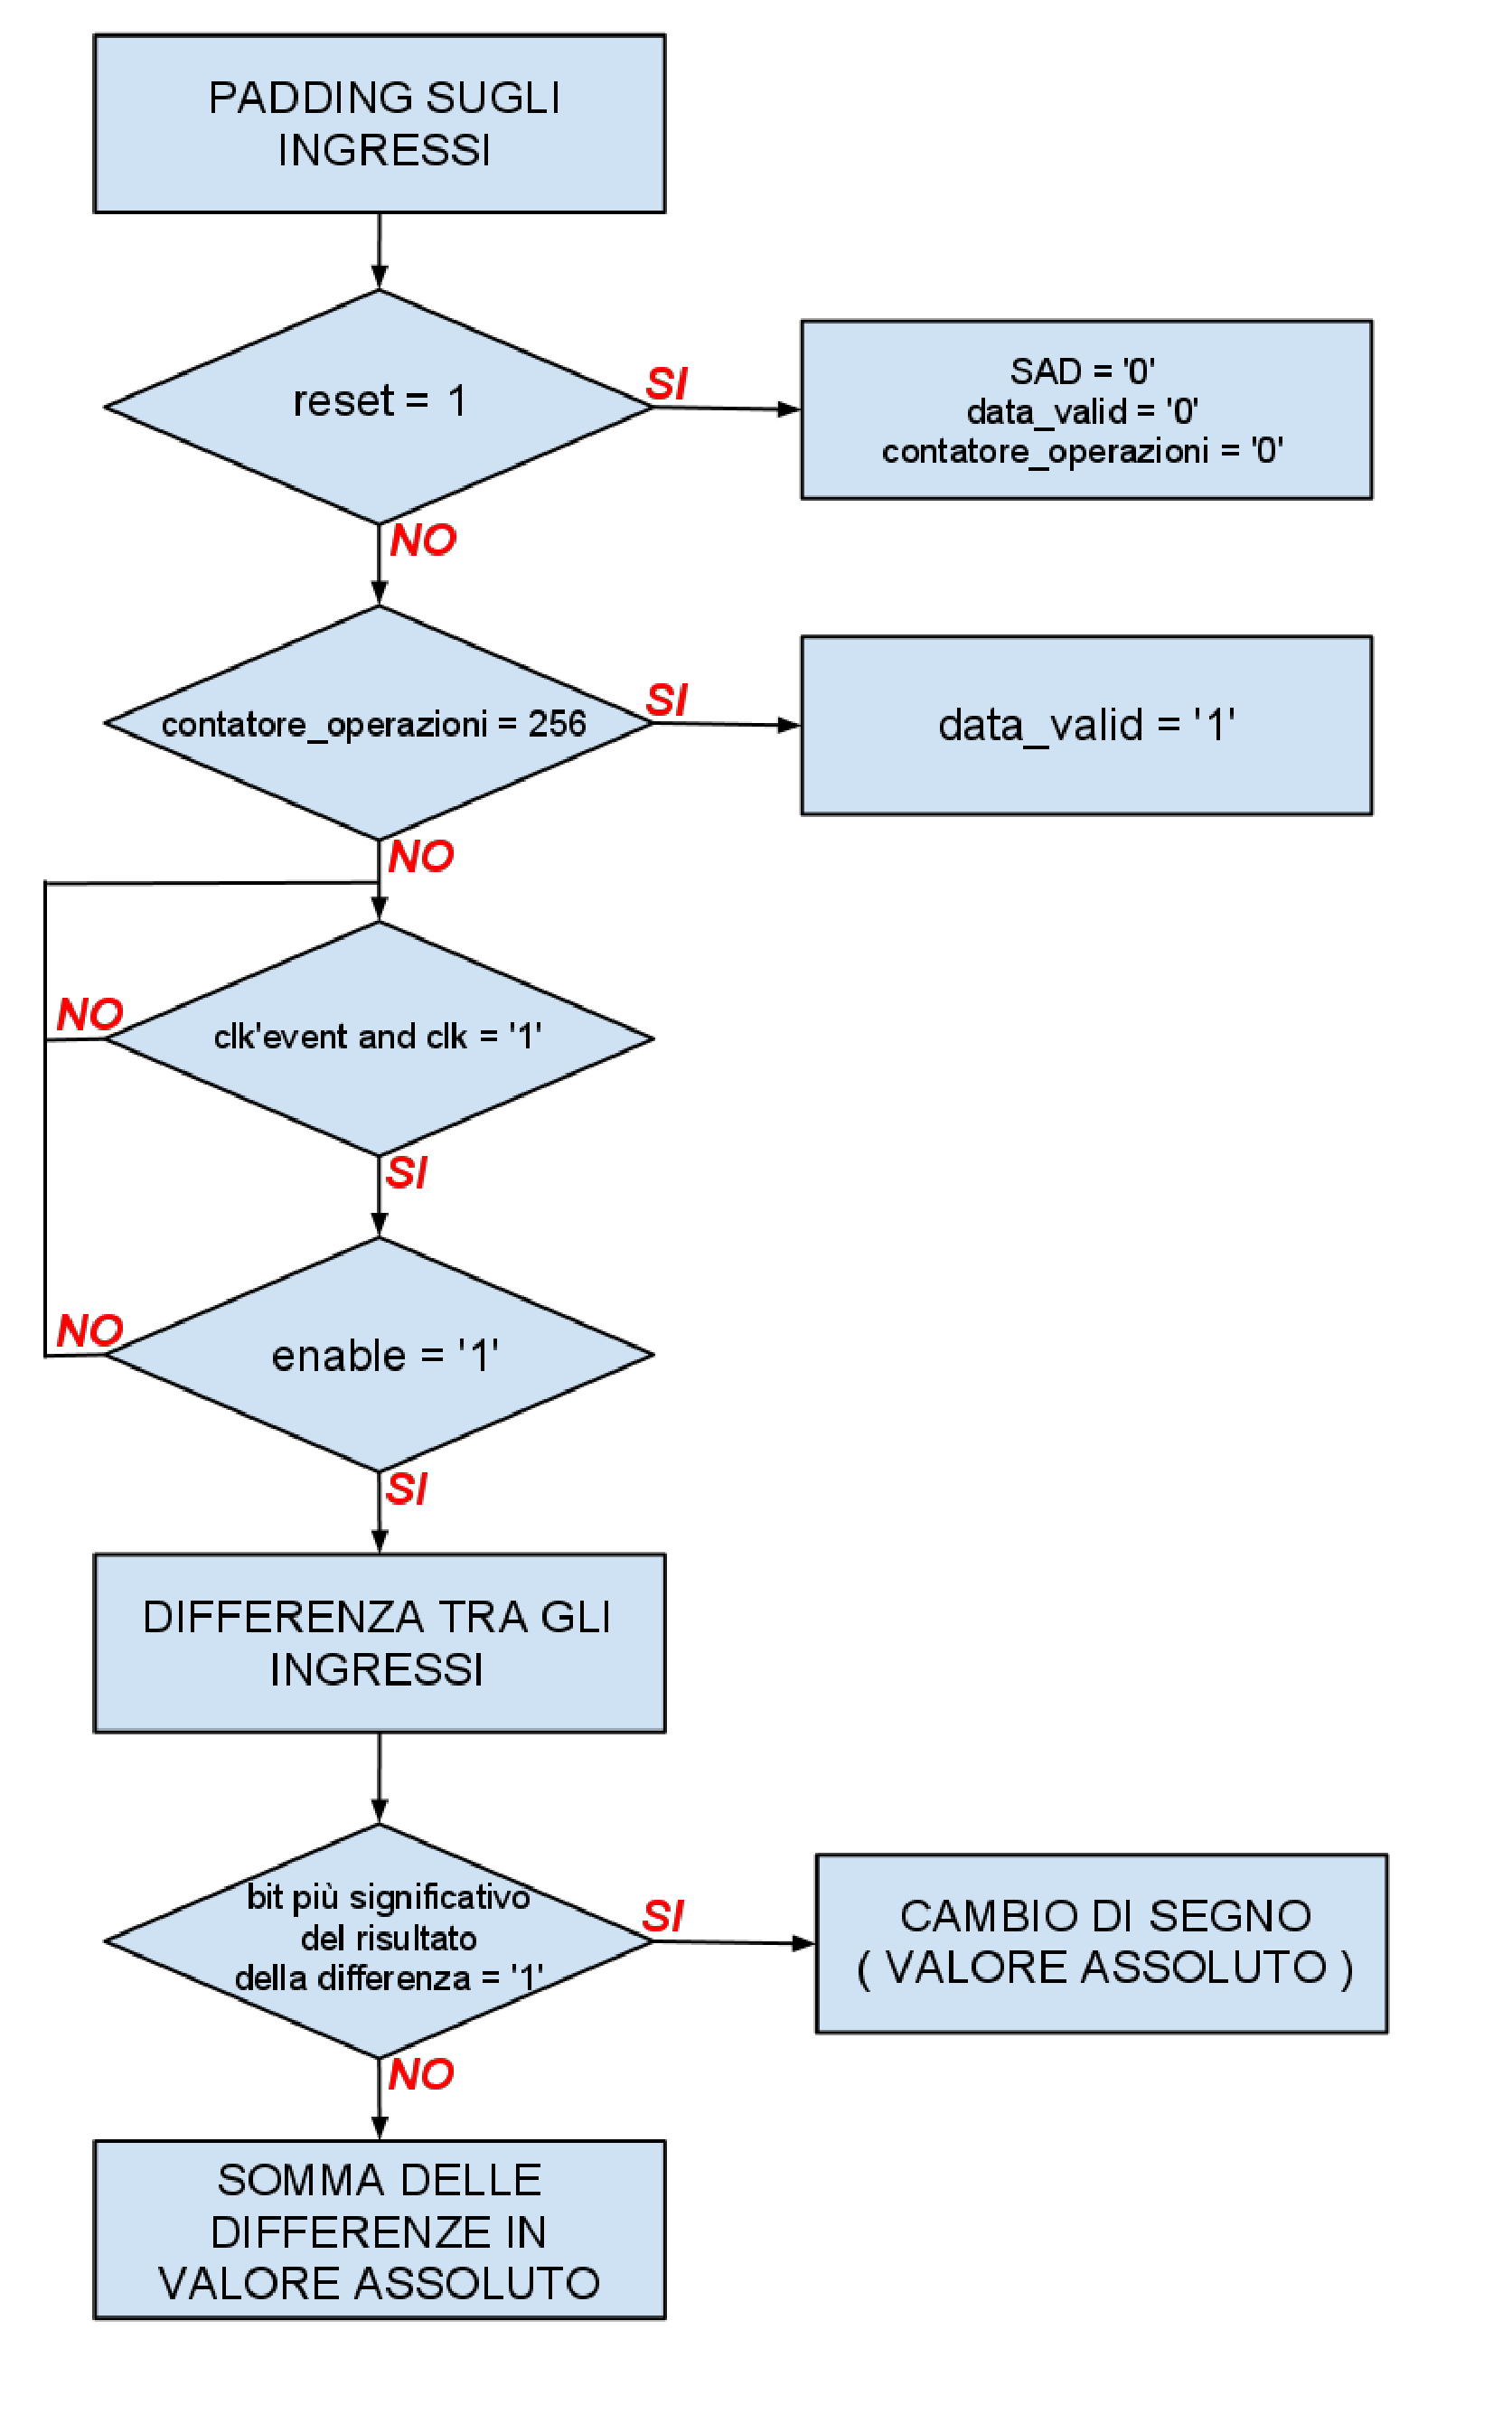
\includegraphics[scale=0.3]{images/sad_behaviour.eps}
\caption{Flusso di progettazione}\label{fig:1}
\end{figure}
\subsection{Caso specifico}
Nel caso specifico i blocchi di immagine monocromatiche hanno dimensioni 16x16 pixel (256 pixel per immagine) ed ogni pixel è un numero intero compreso tra 0 e 255.
Analizzando i dati forniti sono stati dimensionati gli ingressi a 8 bit ($2^8$ = 256), mentre per il dimensionamento dell'uscita si è reso necessario un calcolo preventivo del valore massimo ottenibile come somma dei valori assoluti delle differenze. Precisamente sono necessari, al fine del calcolo, 256 differenze, dove ognuna può avere un valore massimo (in modulo) di 255. Il valore massimo ottenibile in uscita dal circuito con questa configurazione è quindi di 256 (numero di pixel, quindi di differenze)* 255 (valore massimo in modulo di ogni differenza) = 65280, valore che necessita di 16 bit per poter essere rappresentato ($2^{16}$ = 65536).
Il circuito quindi è così strutturato: riceve 2 ingressi \textit{PA} e \textit{PB} a 8 bit, esegue il padding su di essi per uniformarli alla dimensione dell'uscita, esegue la differenza, facendone poi il valore assoluto e somma ad ogni ciclo di clock il valore ottenuto alla somma delle differenze precedenti. Alla 256ima differenza calcolata, il bit \textit{data\_valid} viene settato per segnalare che il calcolo \textit{SAD} è terminato.
\begin{figure}[h!]
\centering
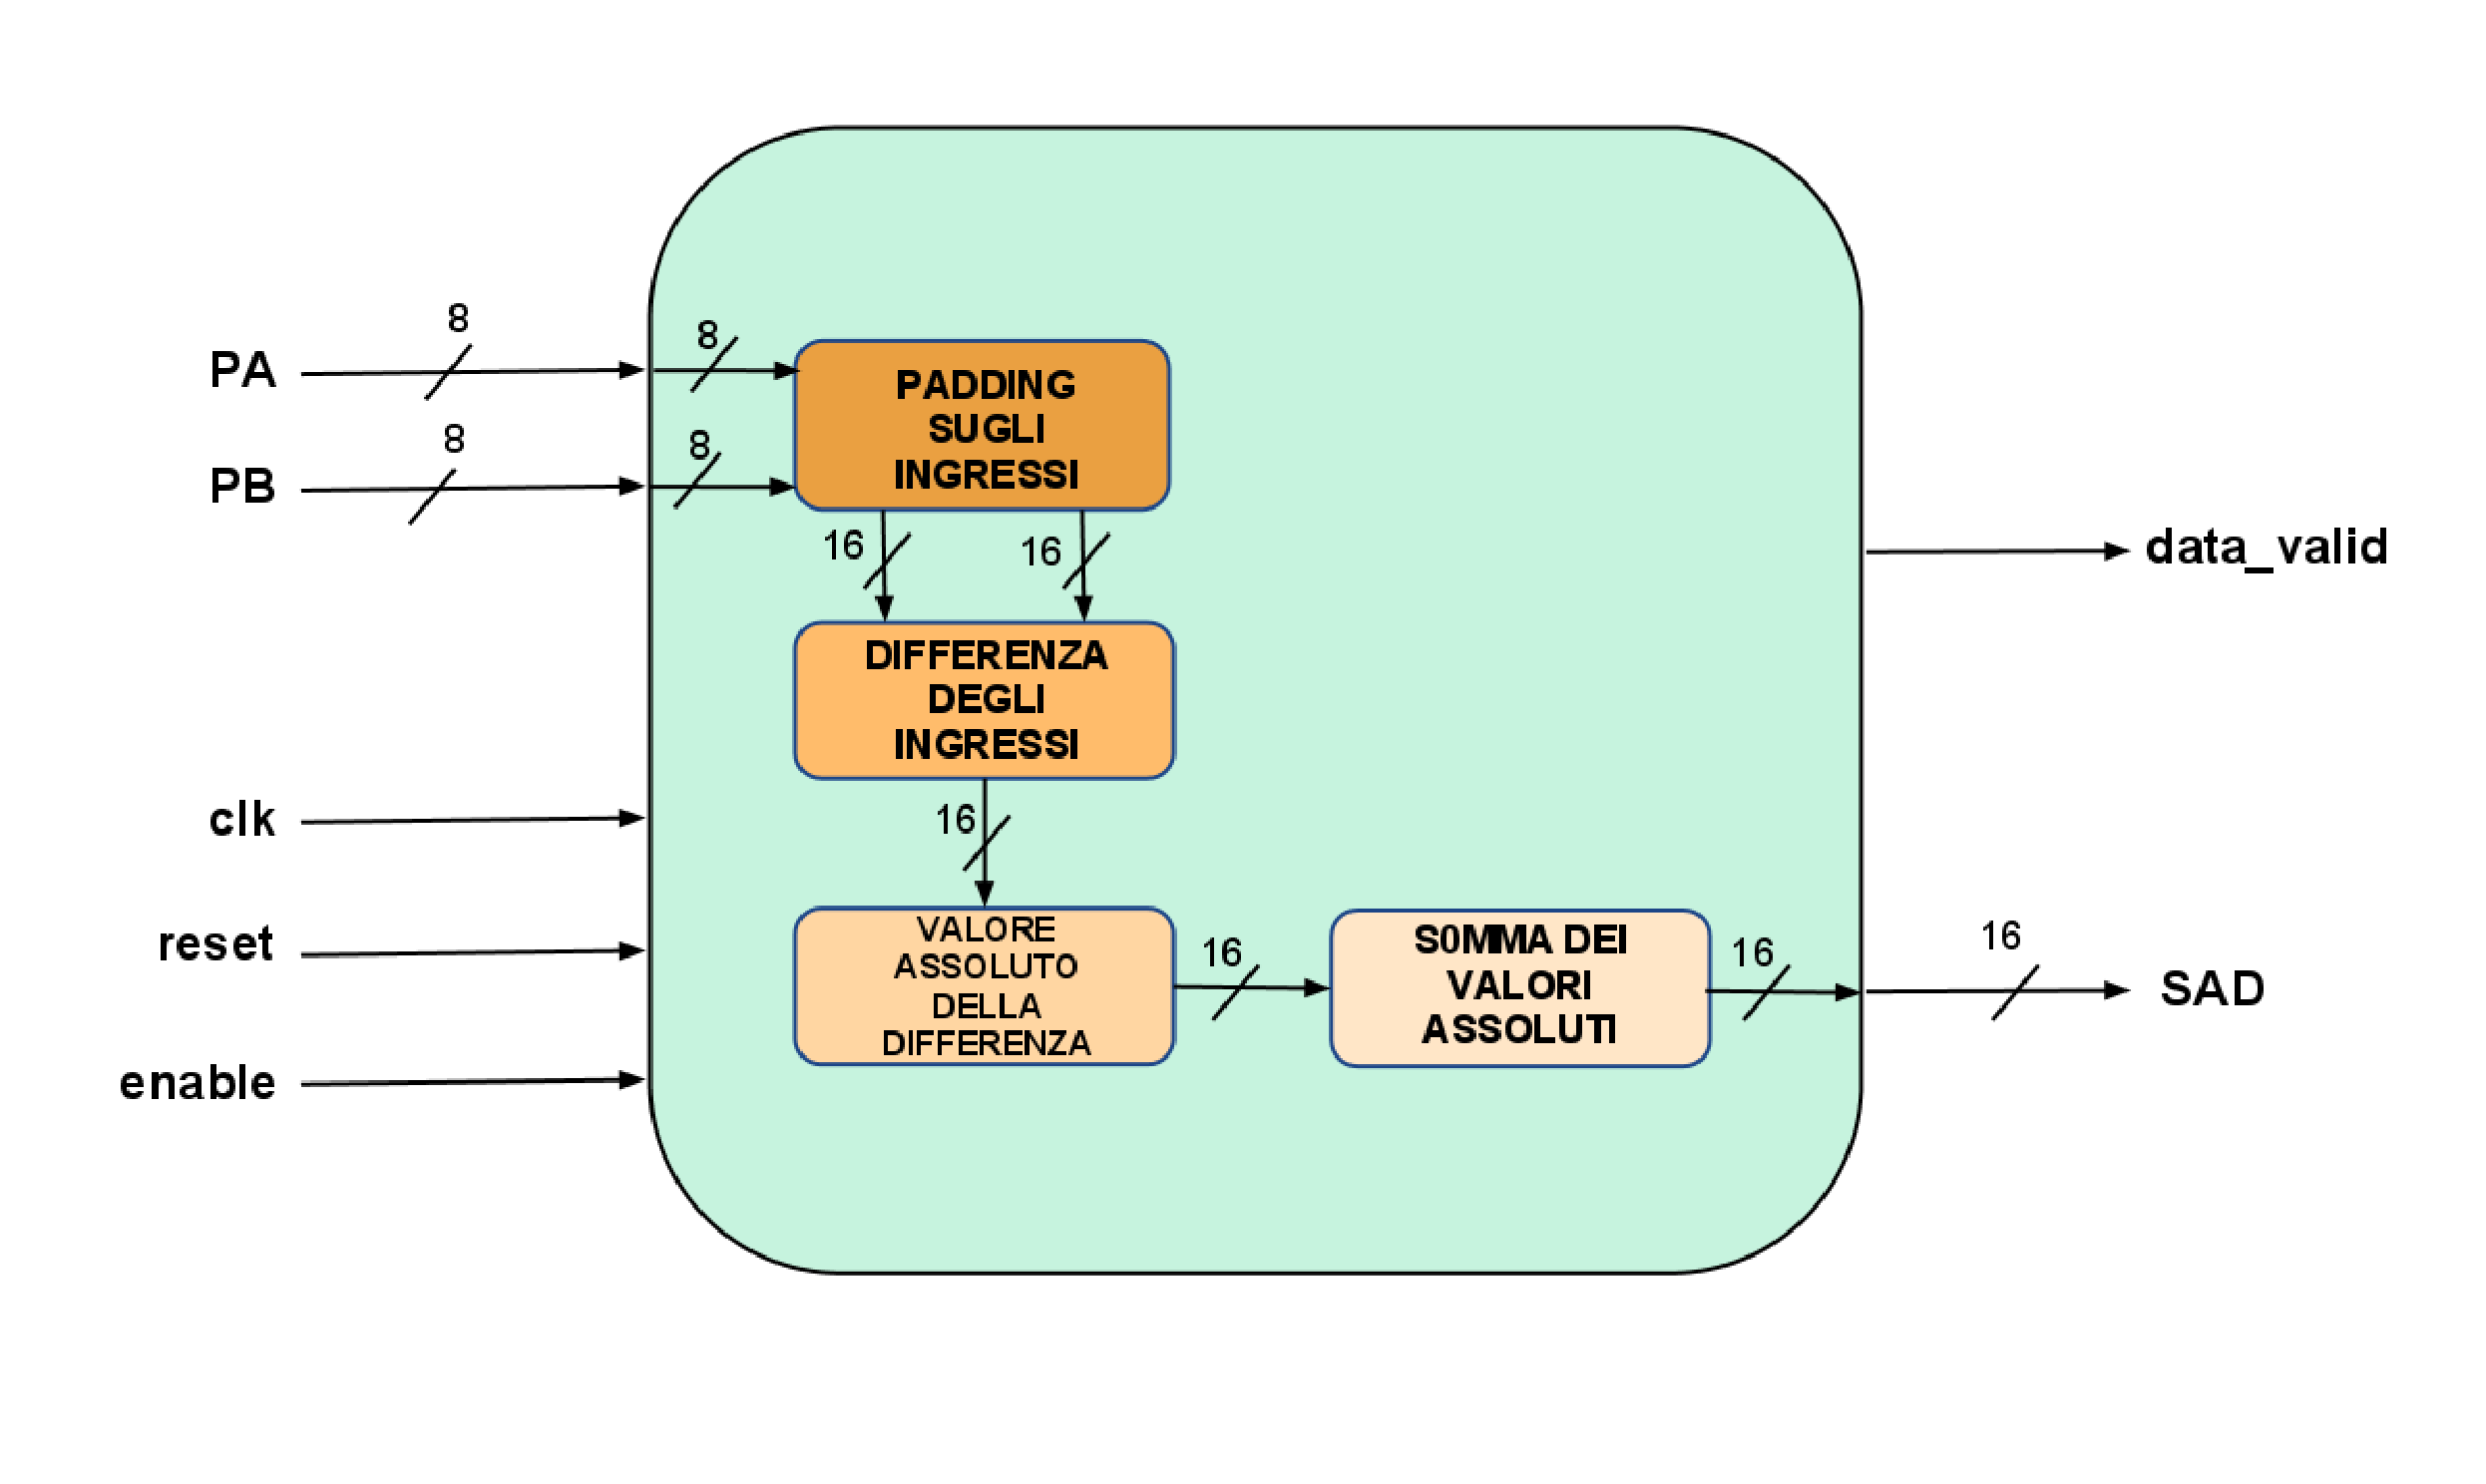
\includegraphics[scale=0.3]{images/sad_general.eps}
\caption{Architettura SAD con ingressi ed uscite specifici}\label{fig:2}
\end{figure}
\subsection{Caso generale}
Nel caso generale invece, ogni immagine è composta da un numero variabile di pixel, precisamente da NxN pixel. I pixel sono anche in questo caso interi compresi tra 0 e 255, di conseguenza gli ingressi sono nuovamente a 8 bit (come prima $2^8$ = 256). Il numero di pixel che compone un'immagine va a variare però il numero di differenze da calcolare, e di conseguenza il numero massimo ottenibile in uscita. Per dimensionare l'uscita \textit{SAD} quindi, si è calcolato il numero massimo ottenibile in funzione di N, secondo la relazione $2^n$ $\geq$ (255 * $N^2$). Questa relazione sta ad indicare che l'uscita deve avere \textit{n} bit, tali che il numero massimo ($2^n$) sia maggiore o uguale al numero massimo ottenuto dalla somma dei moduli delle differenze ovvero 255 (valore massimo del modulo della differenza) * $N^2$ (numero di pixel, quindi di differenze). Facendo una piccola manipolazione matematica della formula sopra descritta, si nota che $n$ $\geq$ $log_2$(255 * $N^2$ ). E' sufficiente quindi fare preventivamente il precedente calcolo, e impostare i valori corretti nel codice relativo al caso specifico, per ottenere il calcolo della \textit{SAD} nel caso generale di immagini composte da NxN pixel.
\begin{figure}[h!]
\centering
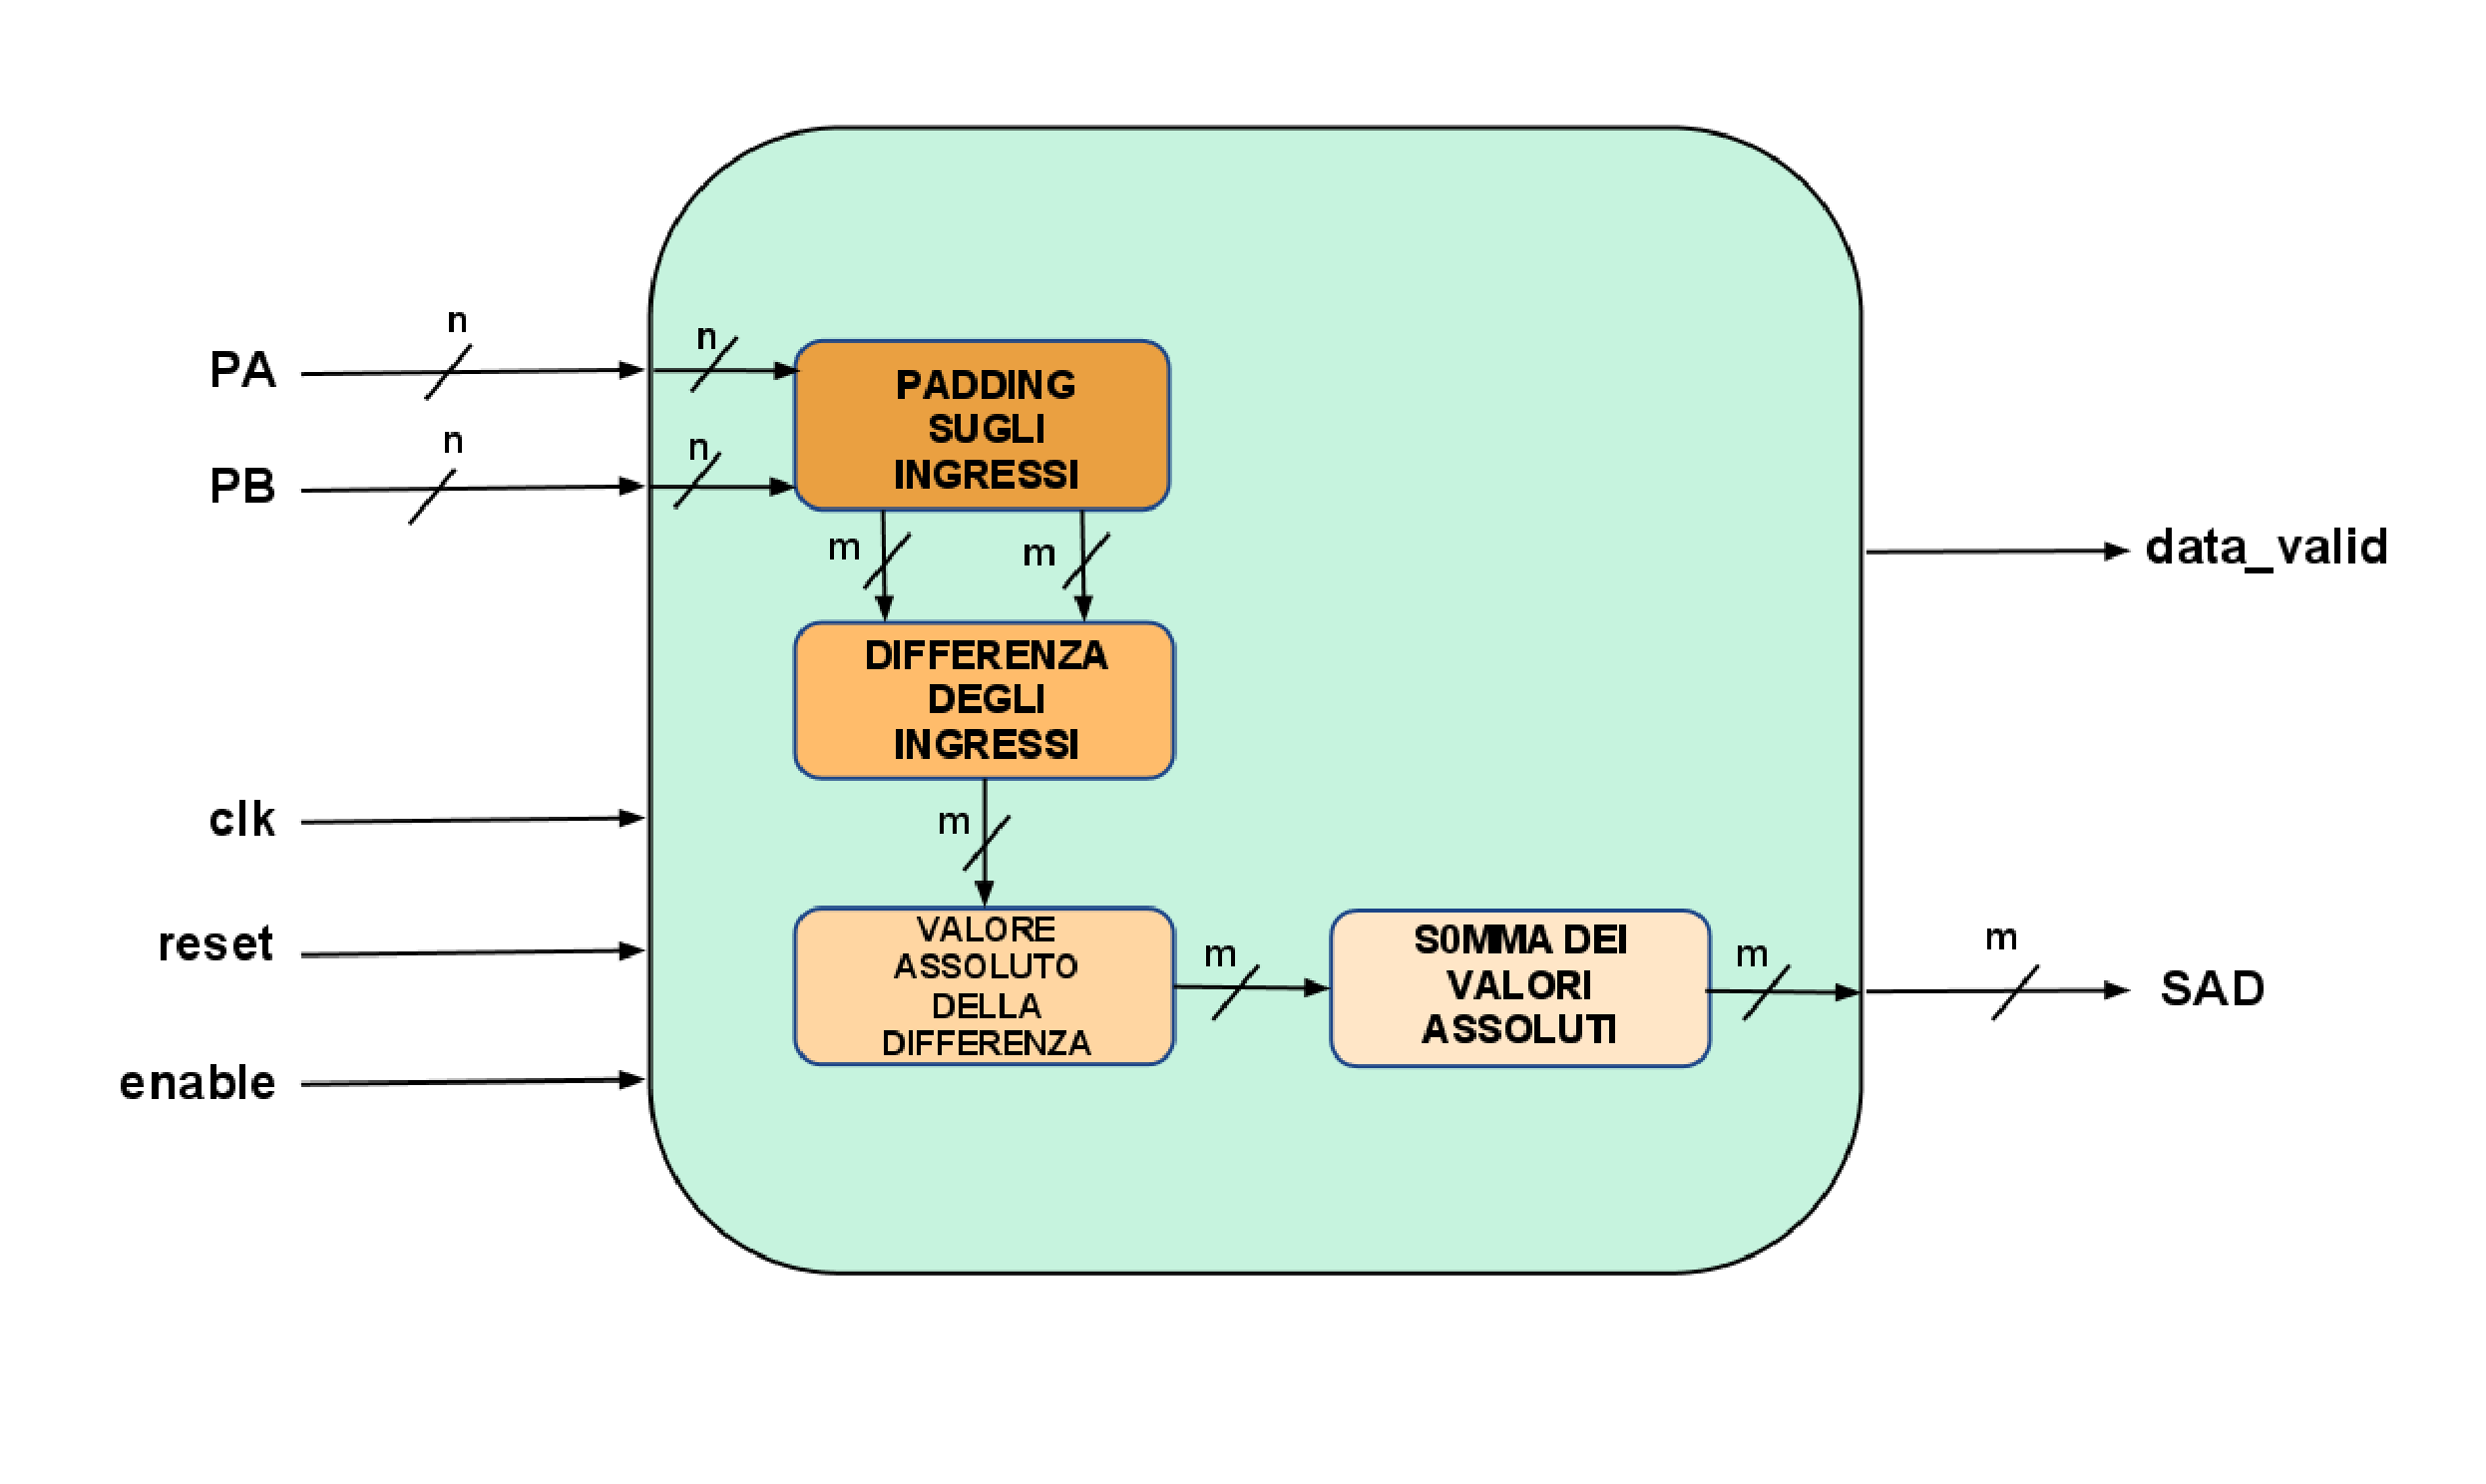
\includegraphics[scale=0.3]{images/sad_general_n.eps}
\caption{Architettura SAD con ingressi ed uscite generici}\label{fig:3}
\end{figure}
\newpage
\section{Analisi VHDL}
\subsection{Codice caso specifico}
{\fontsize{8}{8}
\begin{verbatim}
-------------------------------------------------------------------------------
-- (Behavioral)
--
-- File name	: sad.vhd
-- Purpose	: Calcolo SAD 
--		: somma delle differenze in valore assoluto pixel a pixel
--		: tra due blocchi di immagini monocromatiche A e B
--
--
-- Library   	: IEEE
-- Author(s) 	: Carmine Benedetto, Silvio Bianchi
-- Copyrigth 	: Creative Commons Attribution-ShareAlike 3.0 Unported License
--           	: http://creativecommons.org/licenses/by-sa/3.0/
--
-- Simulator 	: GHDL 0.29 (20100109) [Sokcho edition]
--	     	: GTKWave Analyzer v3.3.10 (w)1999-2010 BSI	
-------------------------------------------------------------------------------
-- Revision List
-- Version	Author					Date		Changes
--
-- 1.0		Carmine Benedetto, Silvio Bianchi	21/09/2011	New version
-------------------------------------------------------------------------------

library IEEE;
use IEEE.numeric_std.all;
use IEEE.std_logic_1164.all;

entity sad_c is

	port(
		PA		: in std_logic_vector(7 downto 0);	-- pixel immagine A
		PB		: in std_logic_vector(7 downto 0);	-- pixel immagine B
		clk		: in std_logic;				-- segnale di clock
		reset		: in std_logic;				-- segnale di reset
		enable		: in std_logic;				-- segnale di enable
		SAD		: out std_logic_vector(15 downto 0);	-- uscita del circuito
		data_valid	: out std_logic				-- segnale data_valid
	);

end sad_c;

architecture behavioural of sad_c is

begin

	sad_proc : process(clk, reset)
	variable pap 	: std_logic_vector(15 downto 0);	-- variabile di appoggio per l'ingresso A
	variable pbp 	: std_logic_vector(15 downto 0);	-- variabile di appoggio per l'ingresso B
	variable cont	: integer;				-- contatore di operazioni
	variable app1 	: std_logic_vector(15 downto 0);	-- variabile di appoggio
	variable app2 	: std_logic_vector(15 downto 0);	-- variabile di appoggio
	variable app3 	: std_logic_vector(15 downto 0);	-- variabile di appoggio

	begin

		-- padding sugli ingressi per renderli uniformi all'uscita
		pap := "00000000" & PA;	
		pbp := "00000000" & PB;

		--  se il segnale di reset e' attivo, azzera le variabili interne e le uscite 
		if (reset = '1') then

			for i in 0 to 15 loop
				app1(i) := '0';
				app2(i) := '0';
				app3(i) := '0';
				SAD(i) <= '0';
			end loop;
			
			data_valid <= '0';
			cont := 0;
		
		-- se sono state effettuate 256 operazioni (16x16 pixel), il calcolo della SAD risulta concluso 
		-- l'uscita data_valid viene settata ad 1
		elsif (cont = 256) then
			data_valid <= '1';

		-- per ogni fronte in salita del clock 
		elsif (clk'event and clk = '1') then

			-- se il segnale di enable e' attivo, effettua la somma delle differenze in valore assoluto
			-- pixel per pixel, altrimenti mantiene lo stato attuale delle variabili e delle uscite
			if(enable = '1') then		
	
				app1 := std_logic_vector( unsigned (pap) - unsigned (pbp) );

				-- se la differenza assume un valore negativo, si effettua un cambio si segno...
				if (app1(8) = '1') then

					app2 := std_logic_vector( -signed (app1) );
				else 
		
					-- ... altrimenti si memorizza il valore della differenza
					app2 := app1;

				end if;

				-- somma del valore assoluto del passo attuale con il valore assoluto dei passi precedenti
				app3 := std_logic_vector( unsigned (app2) + unsigned (app3) );
				SAD <= app3;
				-- si incrementa il contatore di operazioni effettuate
				cont := cont + 1; 

			end if;

		end if;

	end process sad_proc;
		
end behavioural;
\end{verbatim}
}
\begin{quote}
File contenente il codice illustrato: \textit{src/sad.vhd}\\
File di testbench connesso: \textit{src/sad\_test.vhd}
\end{quote}
\newpage
\subsection{Codice caso generale}
{\fontsize{8}{8}
\begin{verbatim}
-------------------------------------------------------------------------------
-- (Behavioral)
--
-- File name	: sad_n.vhd
-- Purpose	: Calcolo SAD 
--		: somma delle differenze in valore assoluto pixel a pixel
--		: tra due blocchi di immagini monocromatiche A e B
--
--
-- Library   	: IEEE
-- Author(s) 	: Carmine Benedetto, Silvio Bianchi
-- Copyrigth 	: Creative Commons Attribution-ShareAlike 3.0 Unported License
--           	: http://creativecommons.org/licenses/by-sa/3.0/
--
-- Simulator 	: GHDL 0.29 (20100109) [Sokcho edition]
--	     	: GTKWave Analyzer v3.3.10 (w)1999-2010 BSI	
-------------------------------------------------------------------------------
-- Revision List
-- Version	Author					Date		Changes
--
-- 1.0		Carmine Benedetto, Silvio Bianchi	21/09/2011	New version
-------------------------------------------------------------------------------

library IEEE;
use IEEE.numeric_std.all;
use IEEE.std_logic_1164.all;

entity sad_c is

	generic (
		npix 	: integer := 32 * 32;	-- numero di pixel dell'immagine
		n 	: integer := 8;		-- dimensione in bit dei pixel in ingresso
		m 	: integer := 18		-- dimensione in bit dell'uscita SAD
	);
	port(
		PA		: in std_logic_vector(n-1 downto 0);	-- pixel immagine A
		PB		: in std_logic_vector(n-1 downto 0);	-- pixel immagine B
		clk		: in std_logic;				-- segnale di clock
		reset		: in std_logic;				-- segnale di reset
		enable		: in std_logic;				-- segnale di enable
		SAD		: out std_logic_vector(m-1 downto 0);	-- uscita del circuito
		data_valid	: out std_logic				-- segnale data_valid
	);

end sad_c;

architecture behavioural of sad_c is

begin

	sad_proc : process(clk, reset)
	variable pap 		: std_logic_vector(m-1 downto 0);	-- variabile di appoggio per l'ingresso A
	variable pbp 		: std_logic_vector(m-1 downto 0);	-- variabile di appoggio per l'ingresso B
	variable cont		: integer;				-- contatore di operazioni
	variable app1		: std_logic_vector(m-1 downto 0);	-- variabile di appoggio
	variable app2 		: std_logic_vector(m-1 downto 0);	-- variabile di appoggio
	variable app3 		: std_logic_vector(m-1 downto 0);	-- variabile di appoggio
	variable padding 	: std_logic_vector(m-n-1 downto 0);	-- variabile per il padding

	begin

		for i in 0 to m-n-1 loop
			padding(i) := '0';
		end loop;

		pap := padding & PA;
		pbp := padding & PB;		
		
		--  se il segnale di reset e' attivo, azzera le variabili interne e le uscite 
		if (reset = '1') then

			for i in 0 to m-1 loop
				app1(i) := '0';
				app2(i) := '0';
				app3(i) := '0';
				SAD(i) <= '0';
			end loop;
			
			data_valid <= '0';
			cont := 0;
		
		-- se sono state effettuate 256 operazioni (16x16 pixel), il calcolo della SAD risulta concluso 
		-- l'uscita data_valid viene settata ad 1
		elsif (cont = npix) then
			data_valid <= '1';

		-- per ogni fronte in salita del clock 
		elsif (clk'event and clk = '1') then

			-- se il segnale di enable e' attivo, effettua la somma delle differenze in valore assoluto
			-- pixel per pixel, altrimenti mantiene lo stato attuale delle variabili e delle uscite
			if(enable = '1') then		
	
				app1 := std_logic_vector( unsigned (pap) - unsigned (pbp) );

				-- se la differenza assume un valore negativo, si effettua un cambio si segno...
				if (app1(n) = '1') then

					app2 := std_logic_vector( -signed (app1) );
				else 
		
					-- ... altrimenti si memorizza il valore della differenza
					app2 := app1;

				end if;

				-- somma del valore assoluto del passo attuale con il valore assoluto dei passi 
				app3 := std_logic_vector( unsigned (app2) + unsigned (app3) );
				SAD <= app3;
				-- si incrementa il contatore di operazioni effettuate
				cont := cont + 1;

			end if;

		end if;

	end process sad_proc;
		
end behavioural;
\end{verbatim}
}
\begin{quote}
In questo caso è stata considerata un'immagine 32 pixel x 32 pixel avente quindi due ingressi ad 8 bit ed un'uscita a 18 bit.\\
File contenente il codice illustrato: \textit{src/sad\_n.vhd}\\
File di testbench connesso: \textit{src/sad\_n\_test.vhd}
\end{quote}
\newpage
Analizziamo adesso ogni singola componente del circuito.
\subsection{Padding sugli ingressi}
La prima operazione che viene eseguita è quella di uniformare la dimensione degli ingressi alla dimensione dell'uscita. Si aggiungono quindi in testa ad ogni ingresso (\textit{PA} e \textit{PB}) tanti 0 quanti sono i bit di differenza tra ingresso e uscita.
{\fontsize{8}{8}
\begin{verbatim}
...

for i in 0 to m-n-1 loop
padding(i) := '0';
end loop;
pap := padding & PA;
pbp := padding & PB;

...
\end{verbatim}
}
\begin{quote}
Dove \textit{m} è il numero di bit dell'uscita, e \textit{n} il numero di bit degli ingressi.
\end{quote}		
\begin{figure}[h!]
\centering
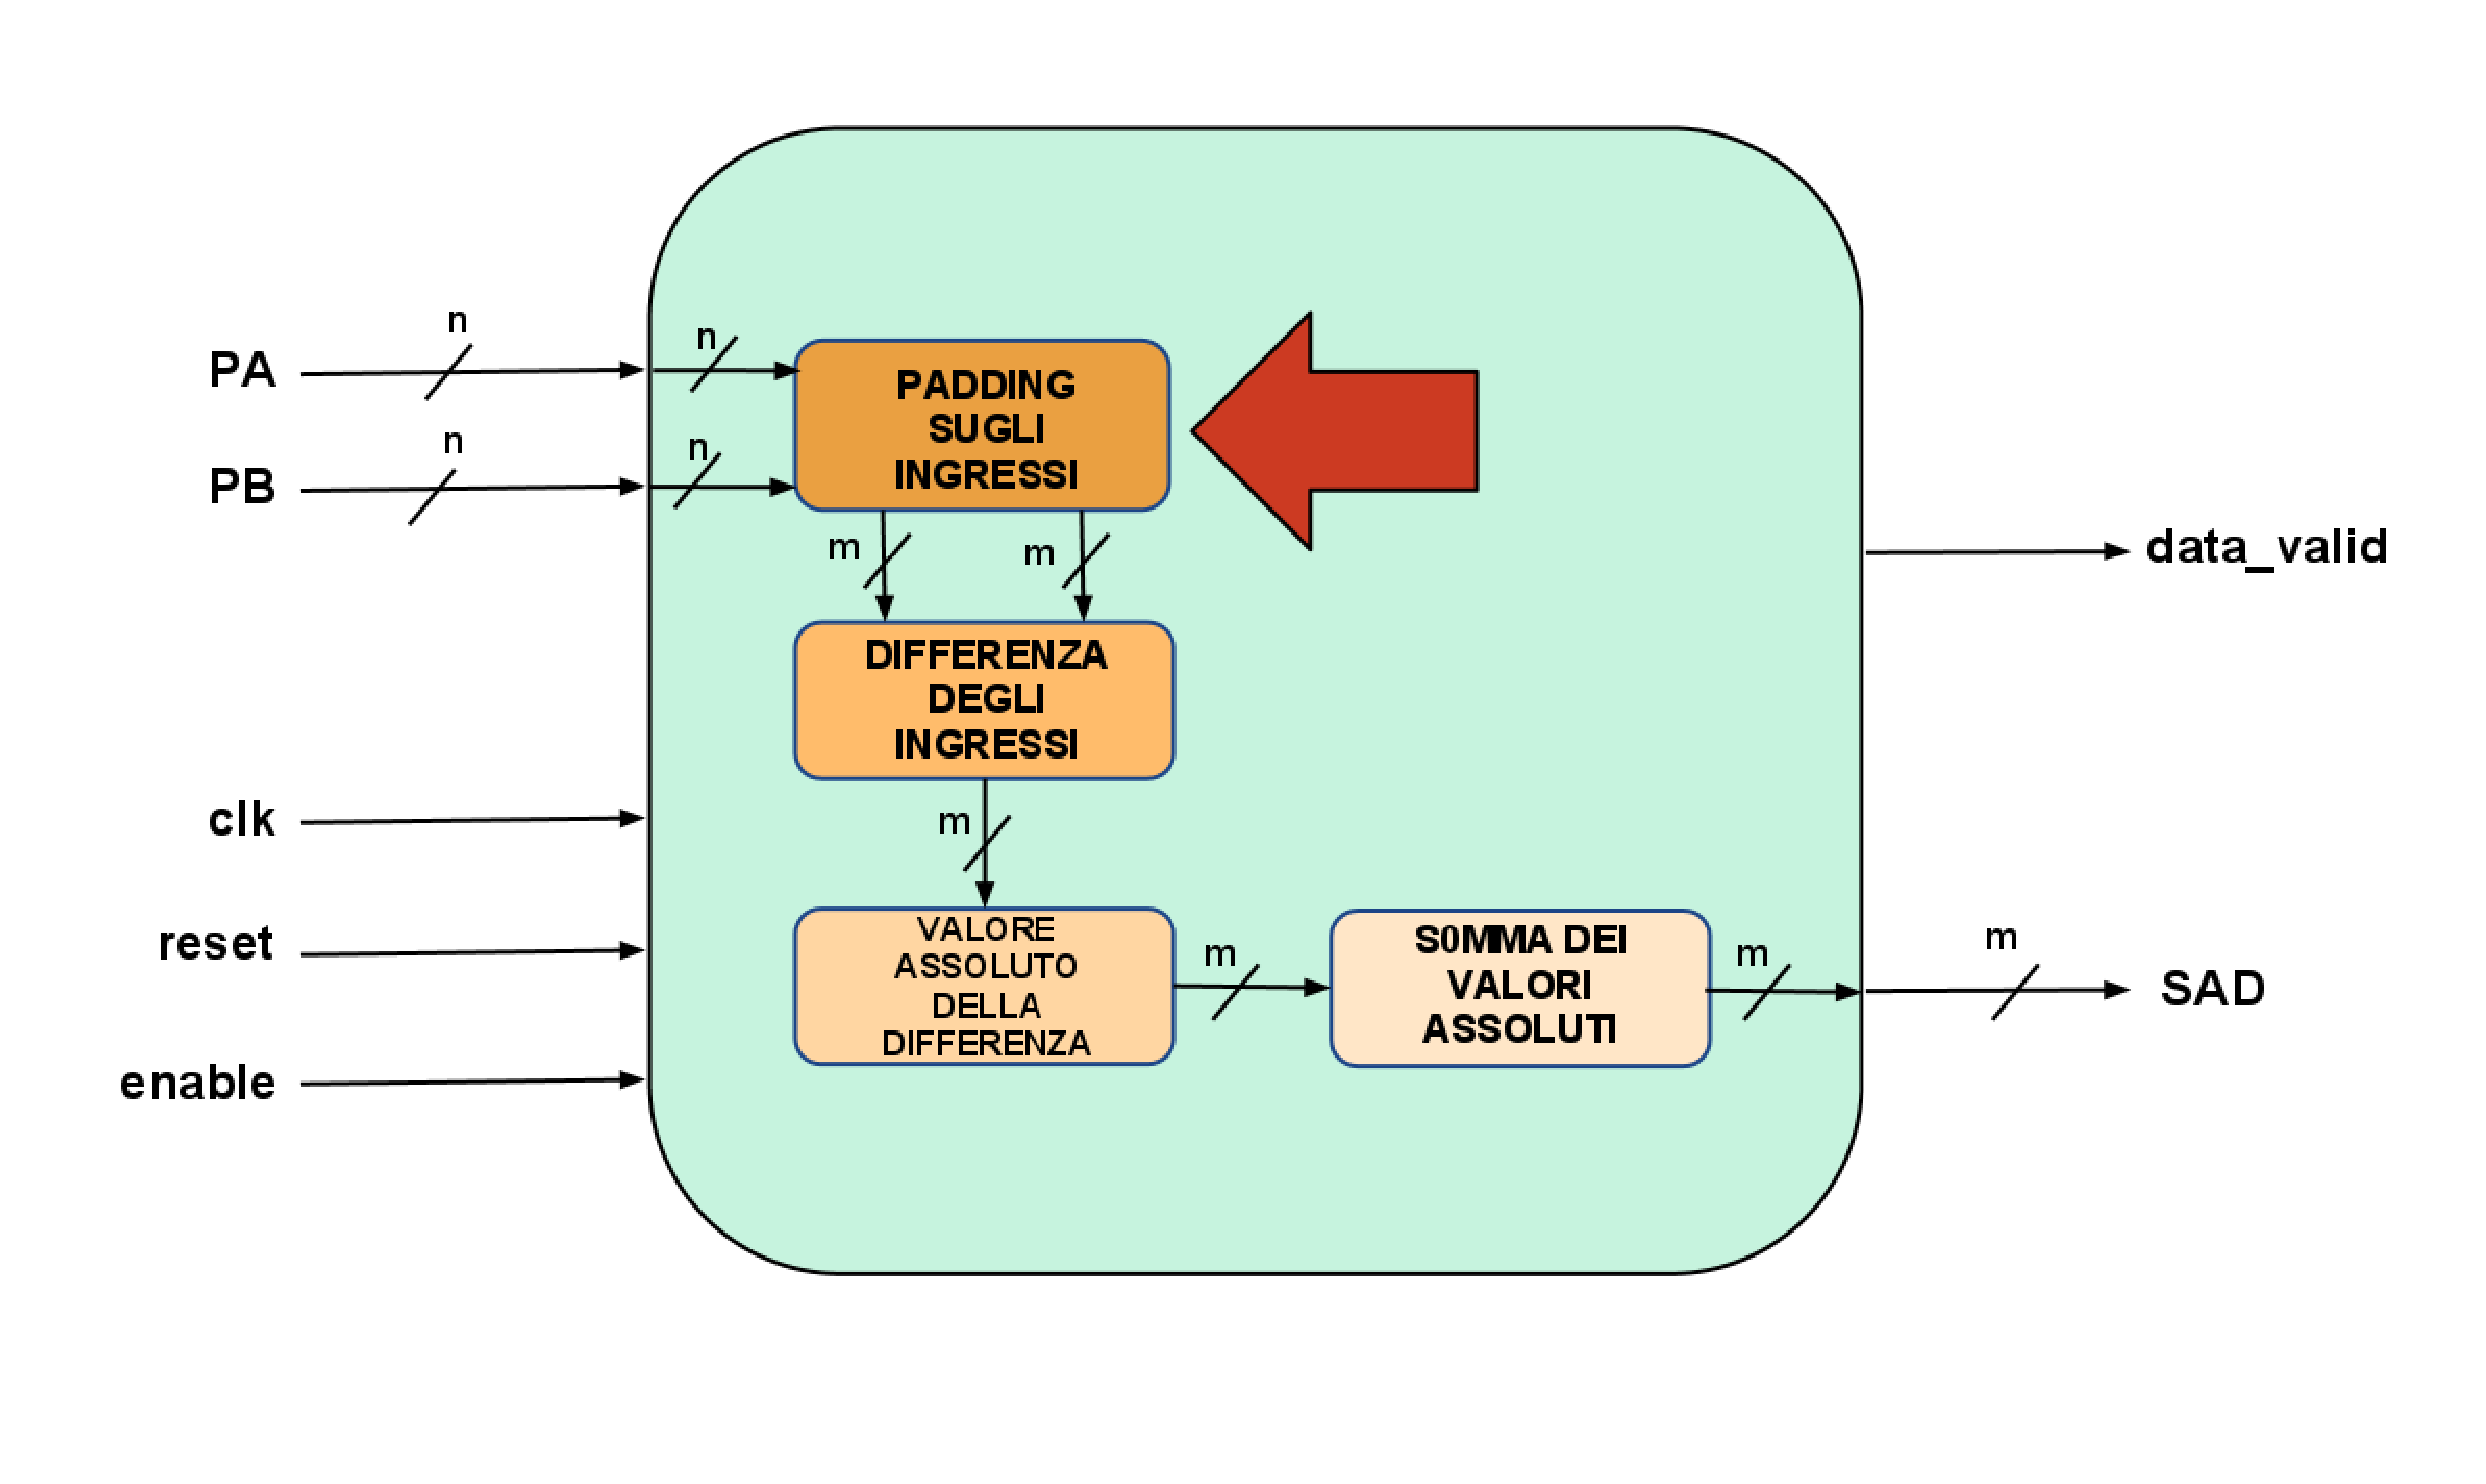
\includegraphics[scale=0.3]{images/padding.eps}
\caption{Modulo Padding}\label{fig:4}
\end{figure}
\newpage
\subsection{Differenza degli ingressi}
In seguito i due ingressi vengono sottratti tra loro, con una semplice operazione di sottrazione, e il risultato messo in una variabile di appoggio \textit{app1}.
{\fontsize{8}{8}
\begin{verbatim}
...

app1 := std_logic_vector( unsigned (pap) - unsigned (pbp) );

...
\end{verbatim}
}
\begin{figure}[h!]
\centering
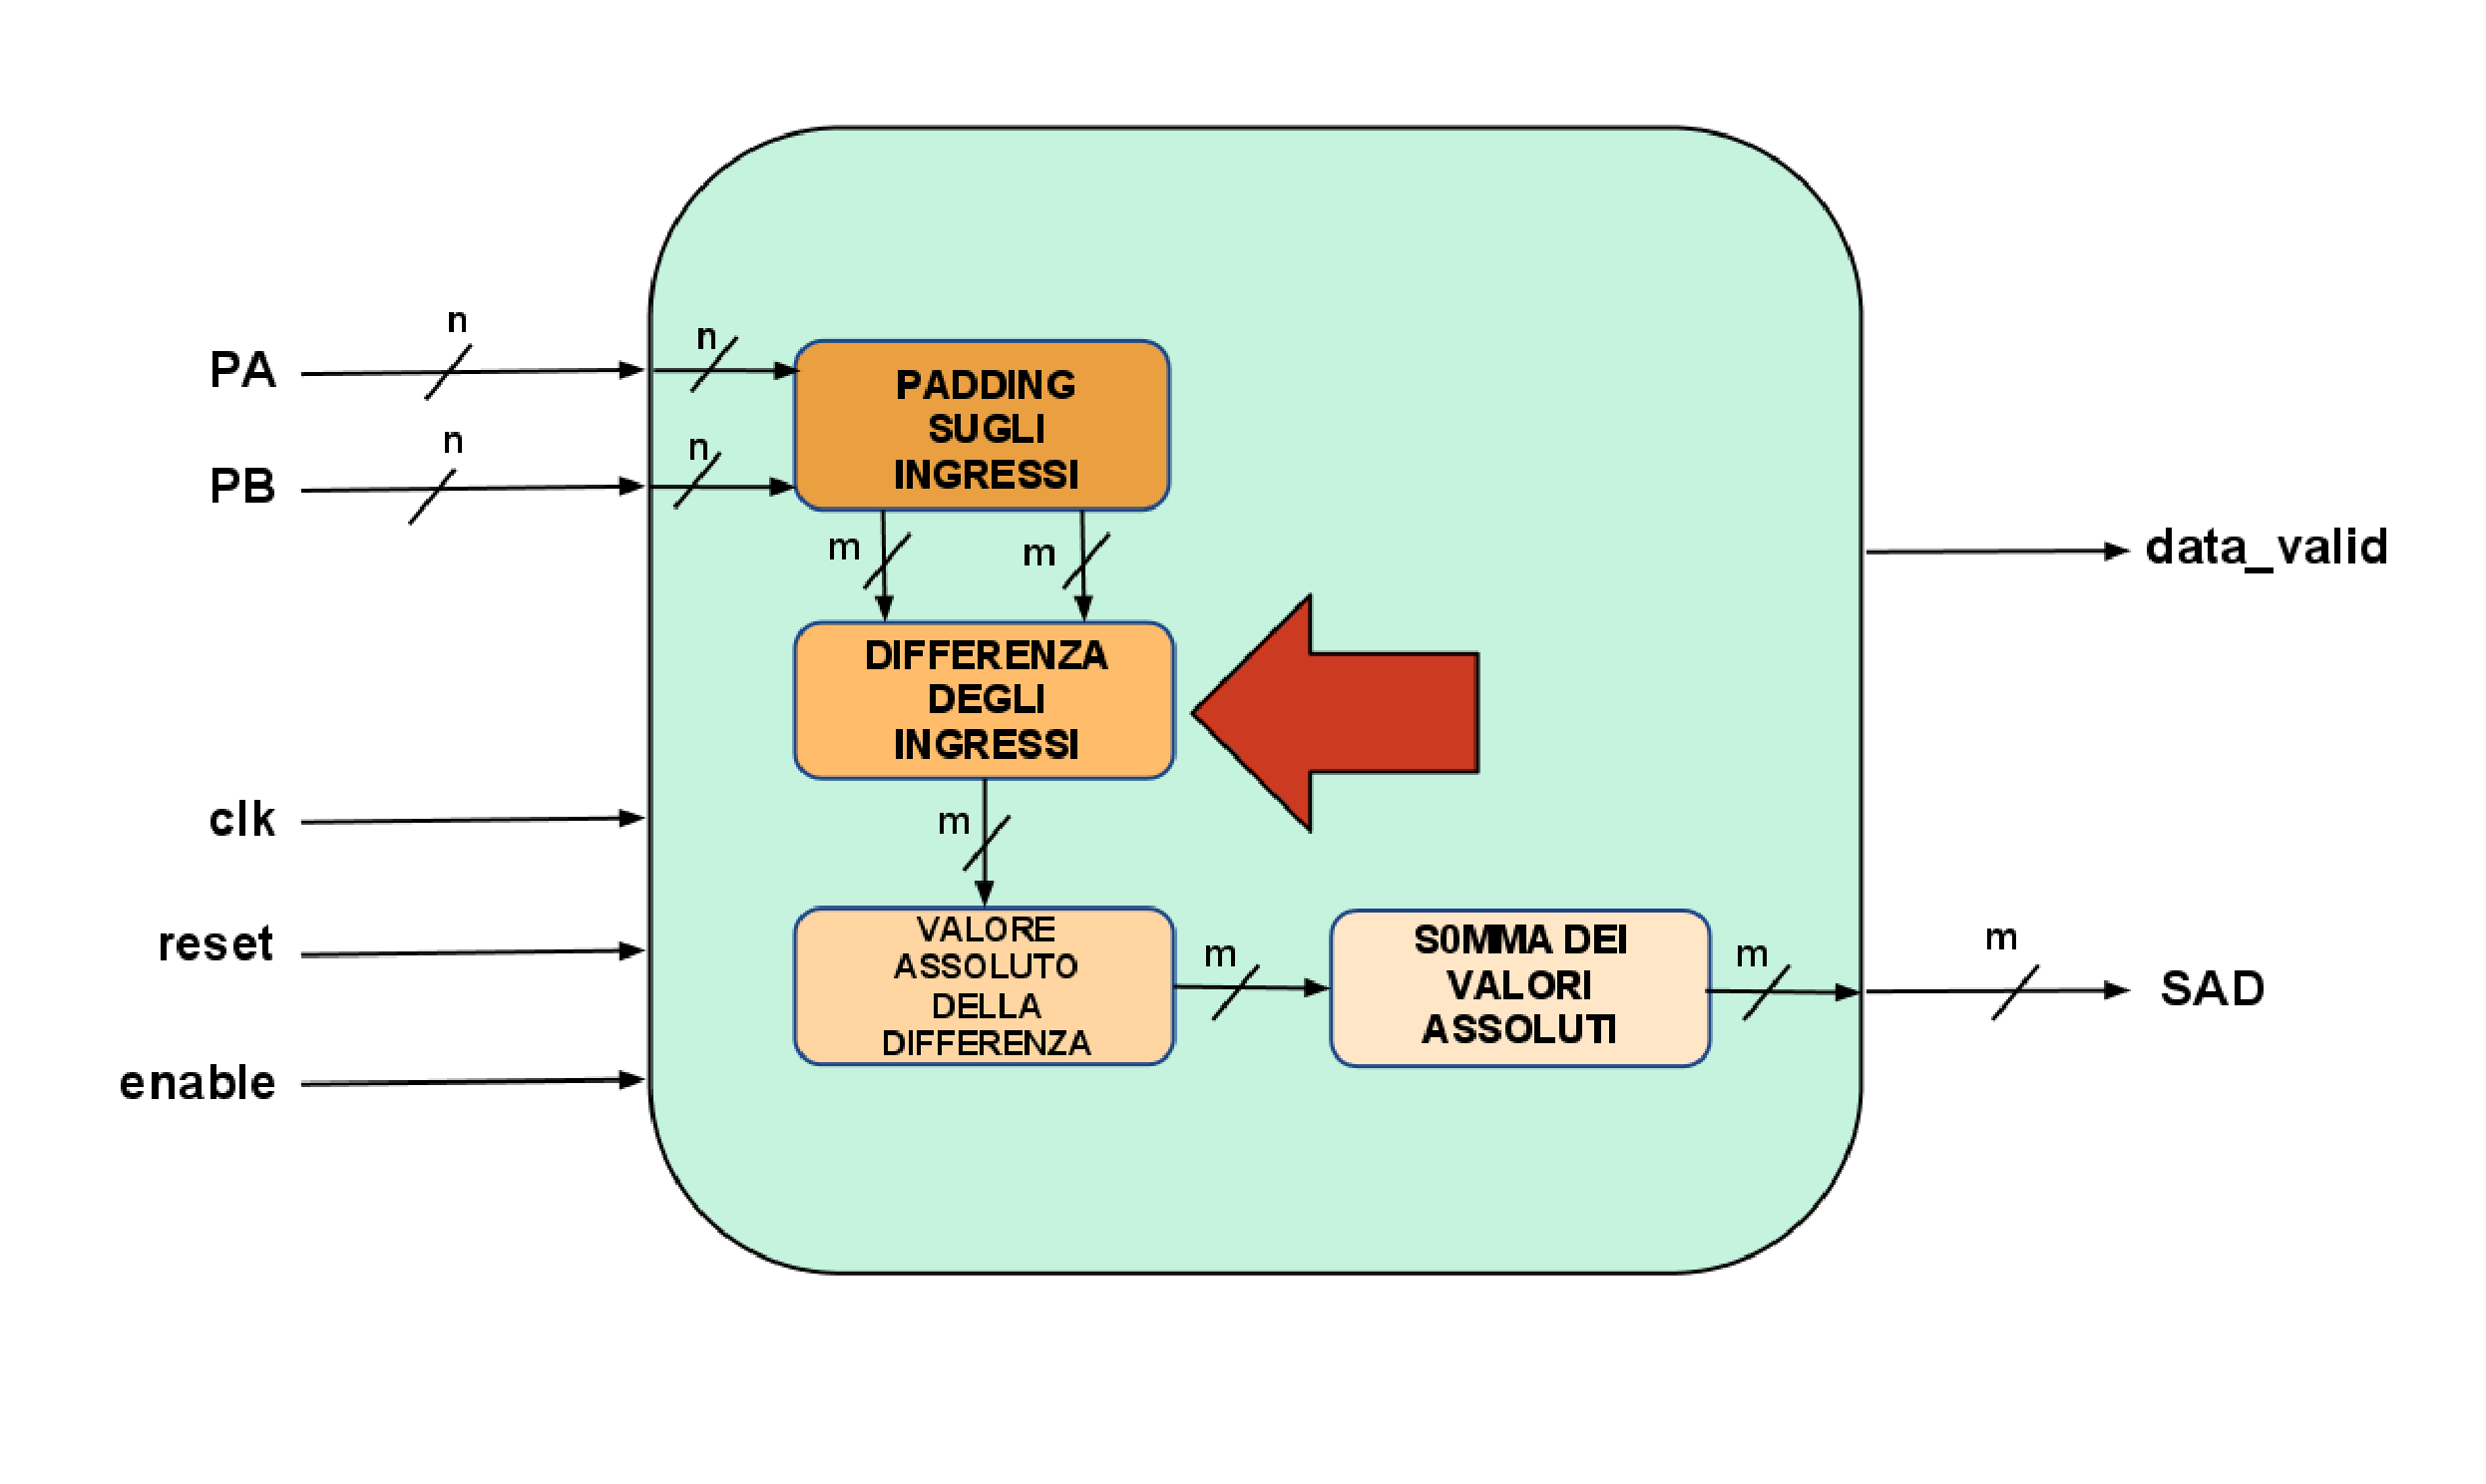
\includegraphics[scale=0.3]{images/differenza.eps}
\caption{Modulo Differenza}\label{fig:5}
\end{figure}
\newpage
\subsection{Valore assoluto della differenza}
La variabile di appoggio \textit{app1} viene analizzata per capire se il risultato della differenza è positivo o negativo (se il \textit{MSB} è settato a 1 il risultato è negativo, positivo altrimenti). Nel caso di risultato negativo è necessario effettuare il cambio di segno del valore ottenuto.
{\fontsize{8}{8}
\begin{verbatim}
...

-- se la differenza assume un valore negativo, si effettua un cambio si segno...
if (app1(n) = '1') then
app2 := std_logic_vector( -signed (app1) );
else 		
-- ... altrimenti si memorizza il valore della differenza
app2 := app1;
end if;

...
\end{verbatim}
}
\begin{figure}[h!]
\centering
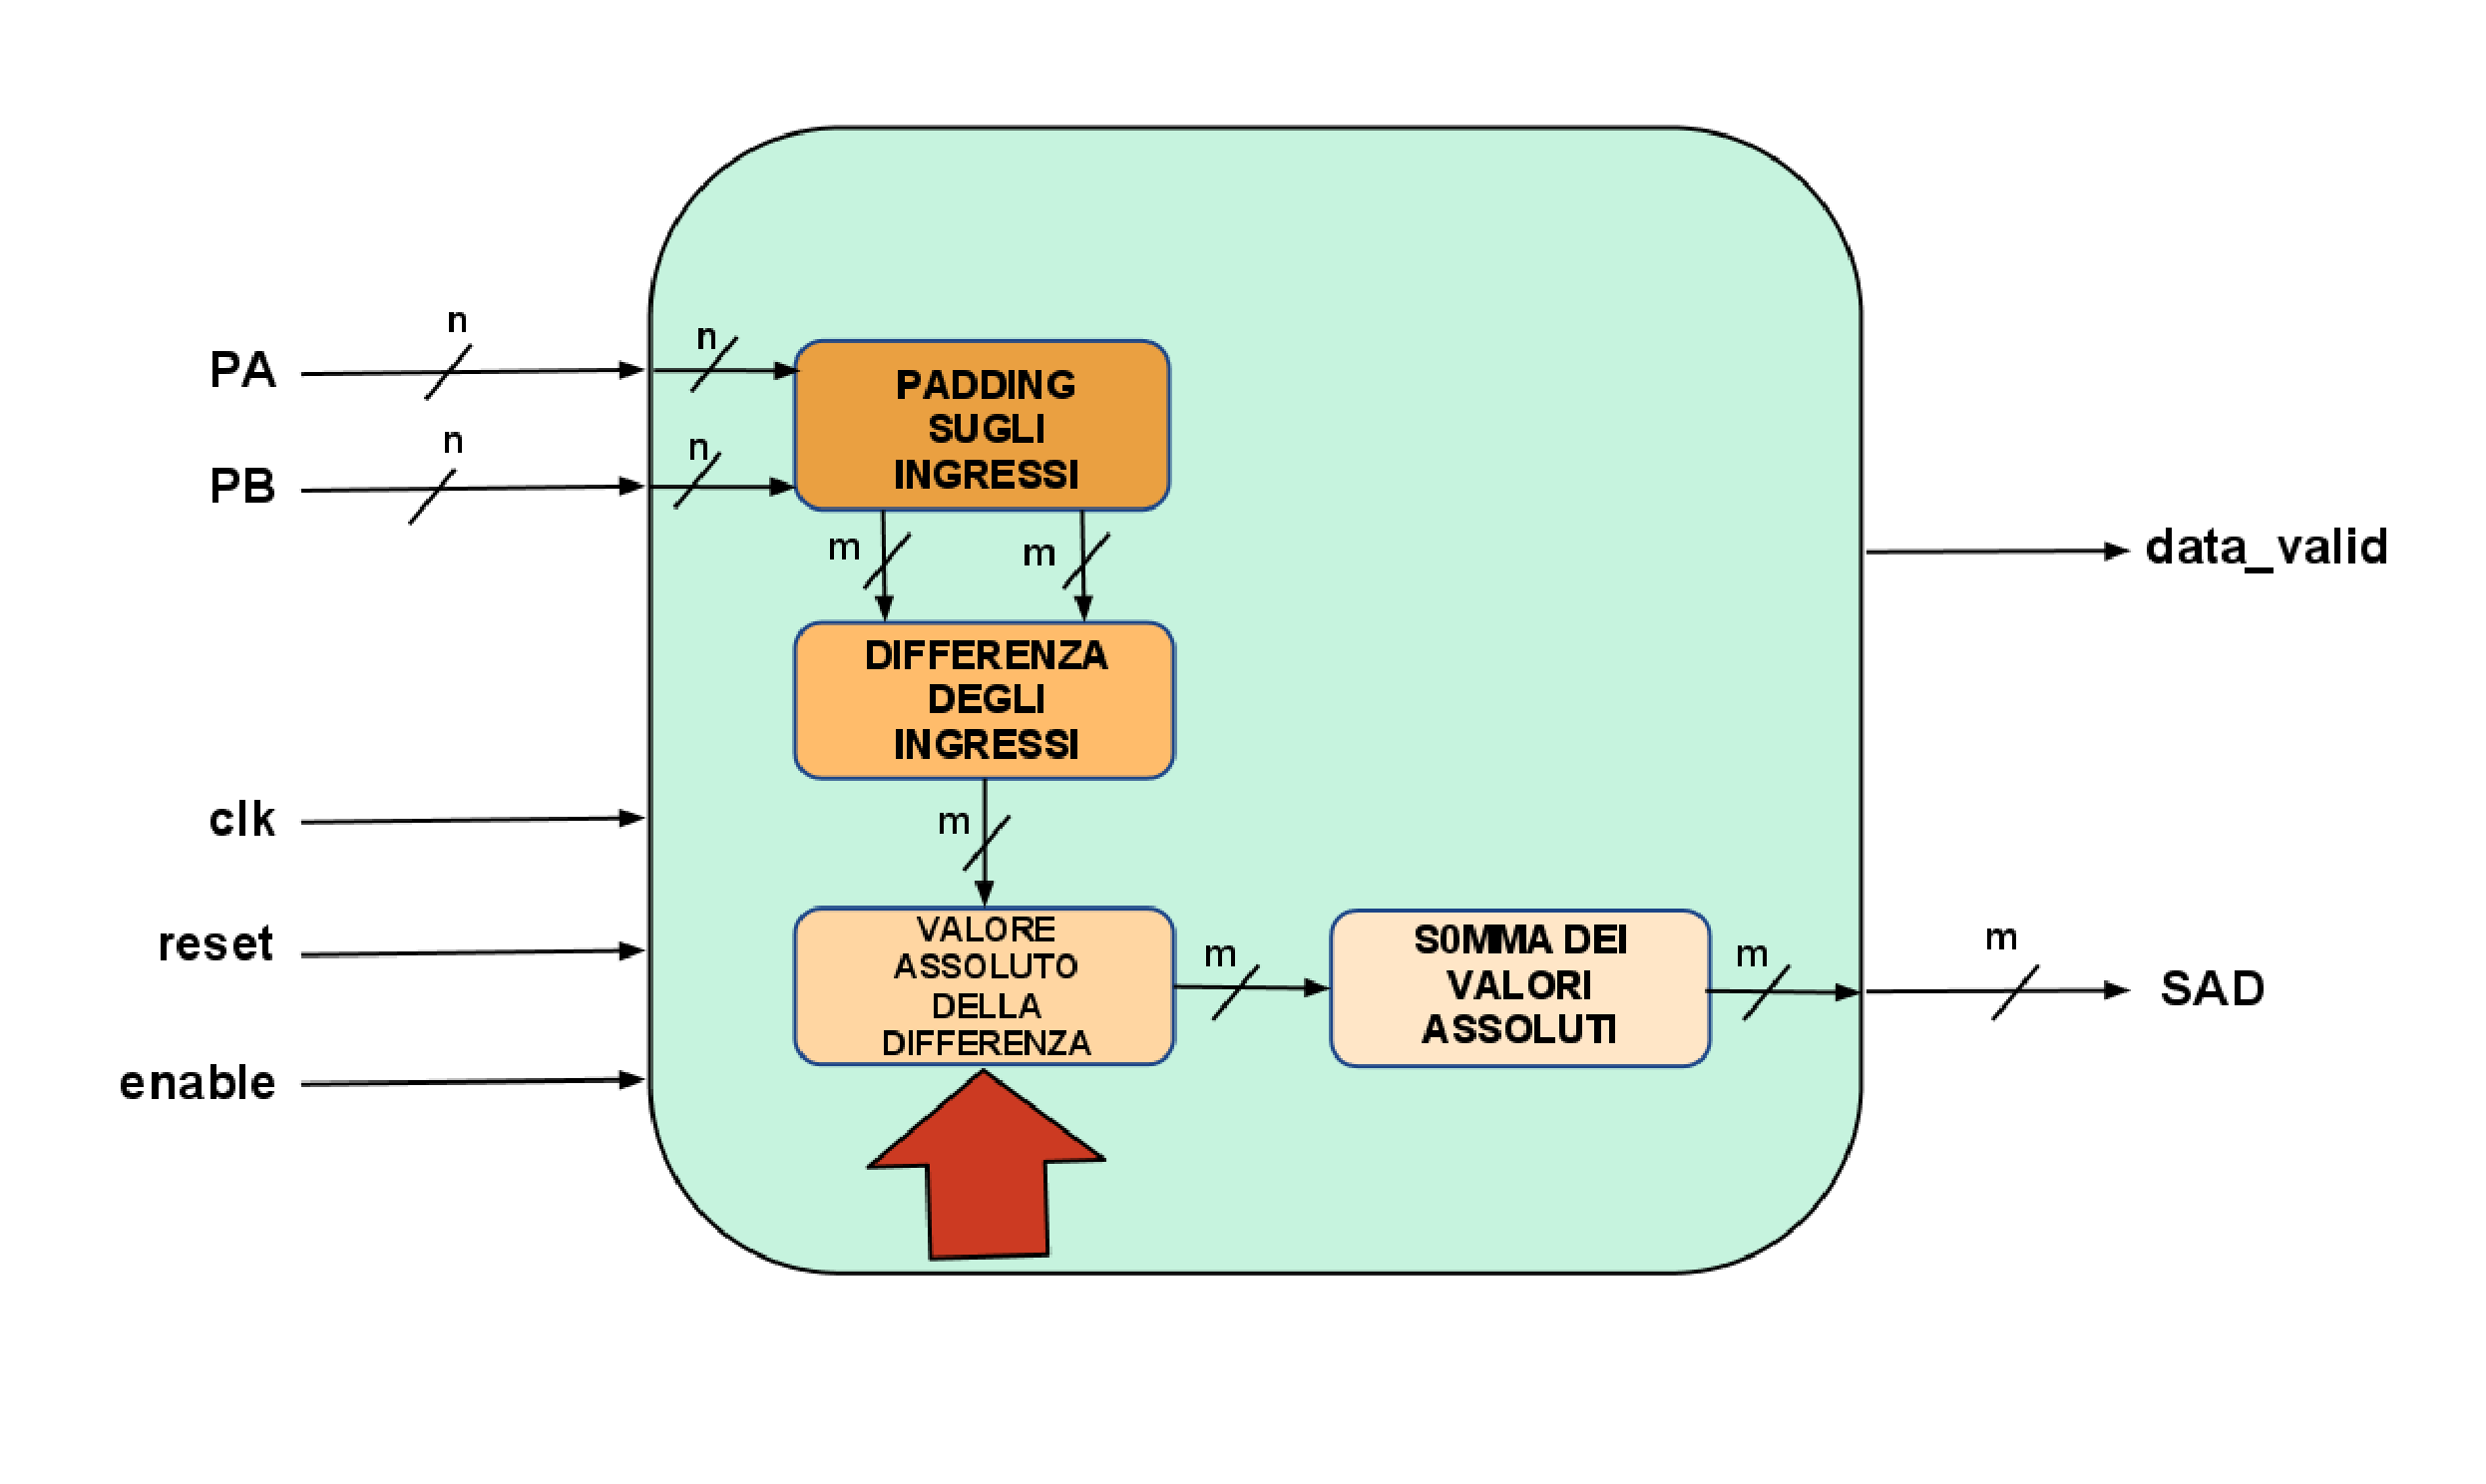
\includegraphics[scale=0.3]{images/abs.eps}
\caption{Modulo Valore Assoluto}\label{fig:6}
\end{figure}
\newpage
\subsection{Somma dei valori assoluti}
L'ultimo elemento del circuito è quello che somma ad ogni passo il modulo della differenza ottenuta in quel passo con la somma dei moduli delle differenze di tutti passi precedenti, mettendo poi tale valore nell'uscita \textit{SAD}.
{\fontsize{8}{8}
\begin{verbatim}
...

-- somma del valore assoluto del passo attuale con il valore assoluto dei passi precedenti
app3 := std_logic_vector( unsigned (app2) + unsigned (app3) );
SAD <= app3;

...
\end{verbatim}
}
\begin{figure}[h!]
\centering
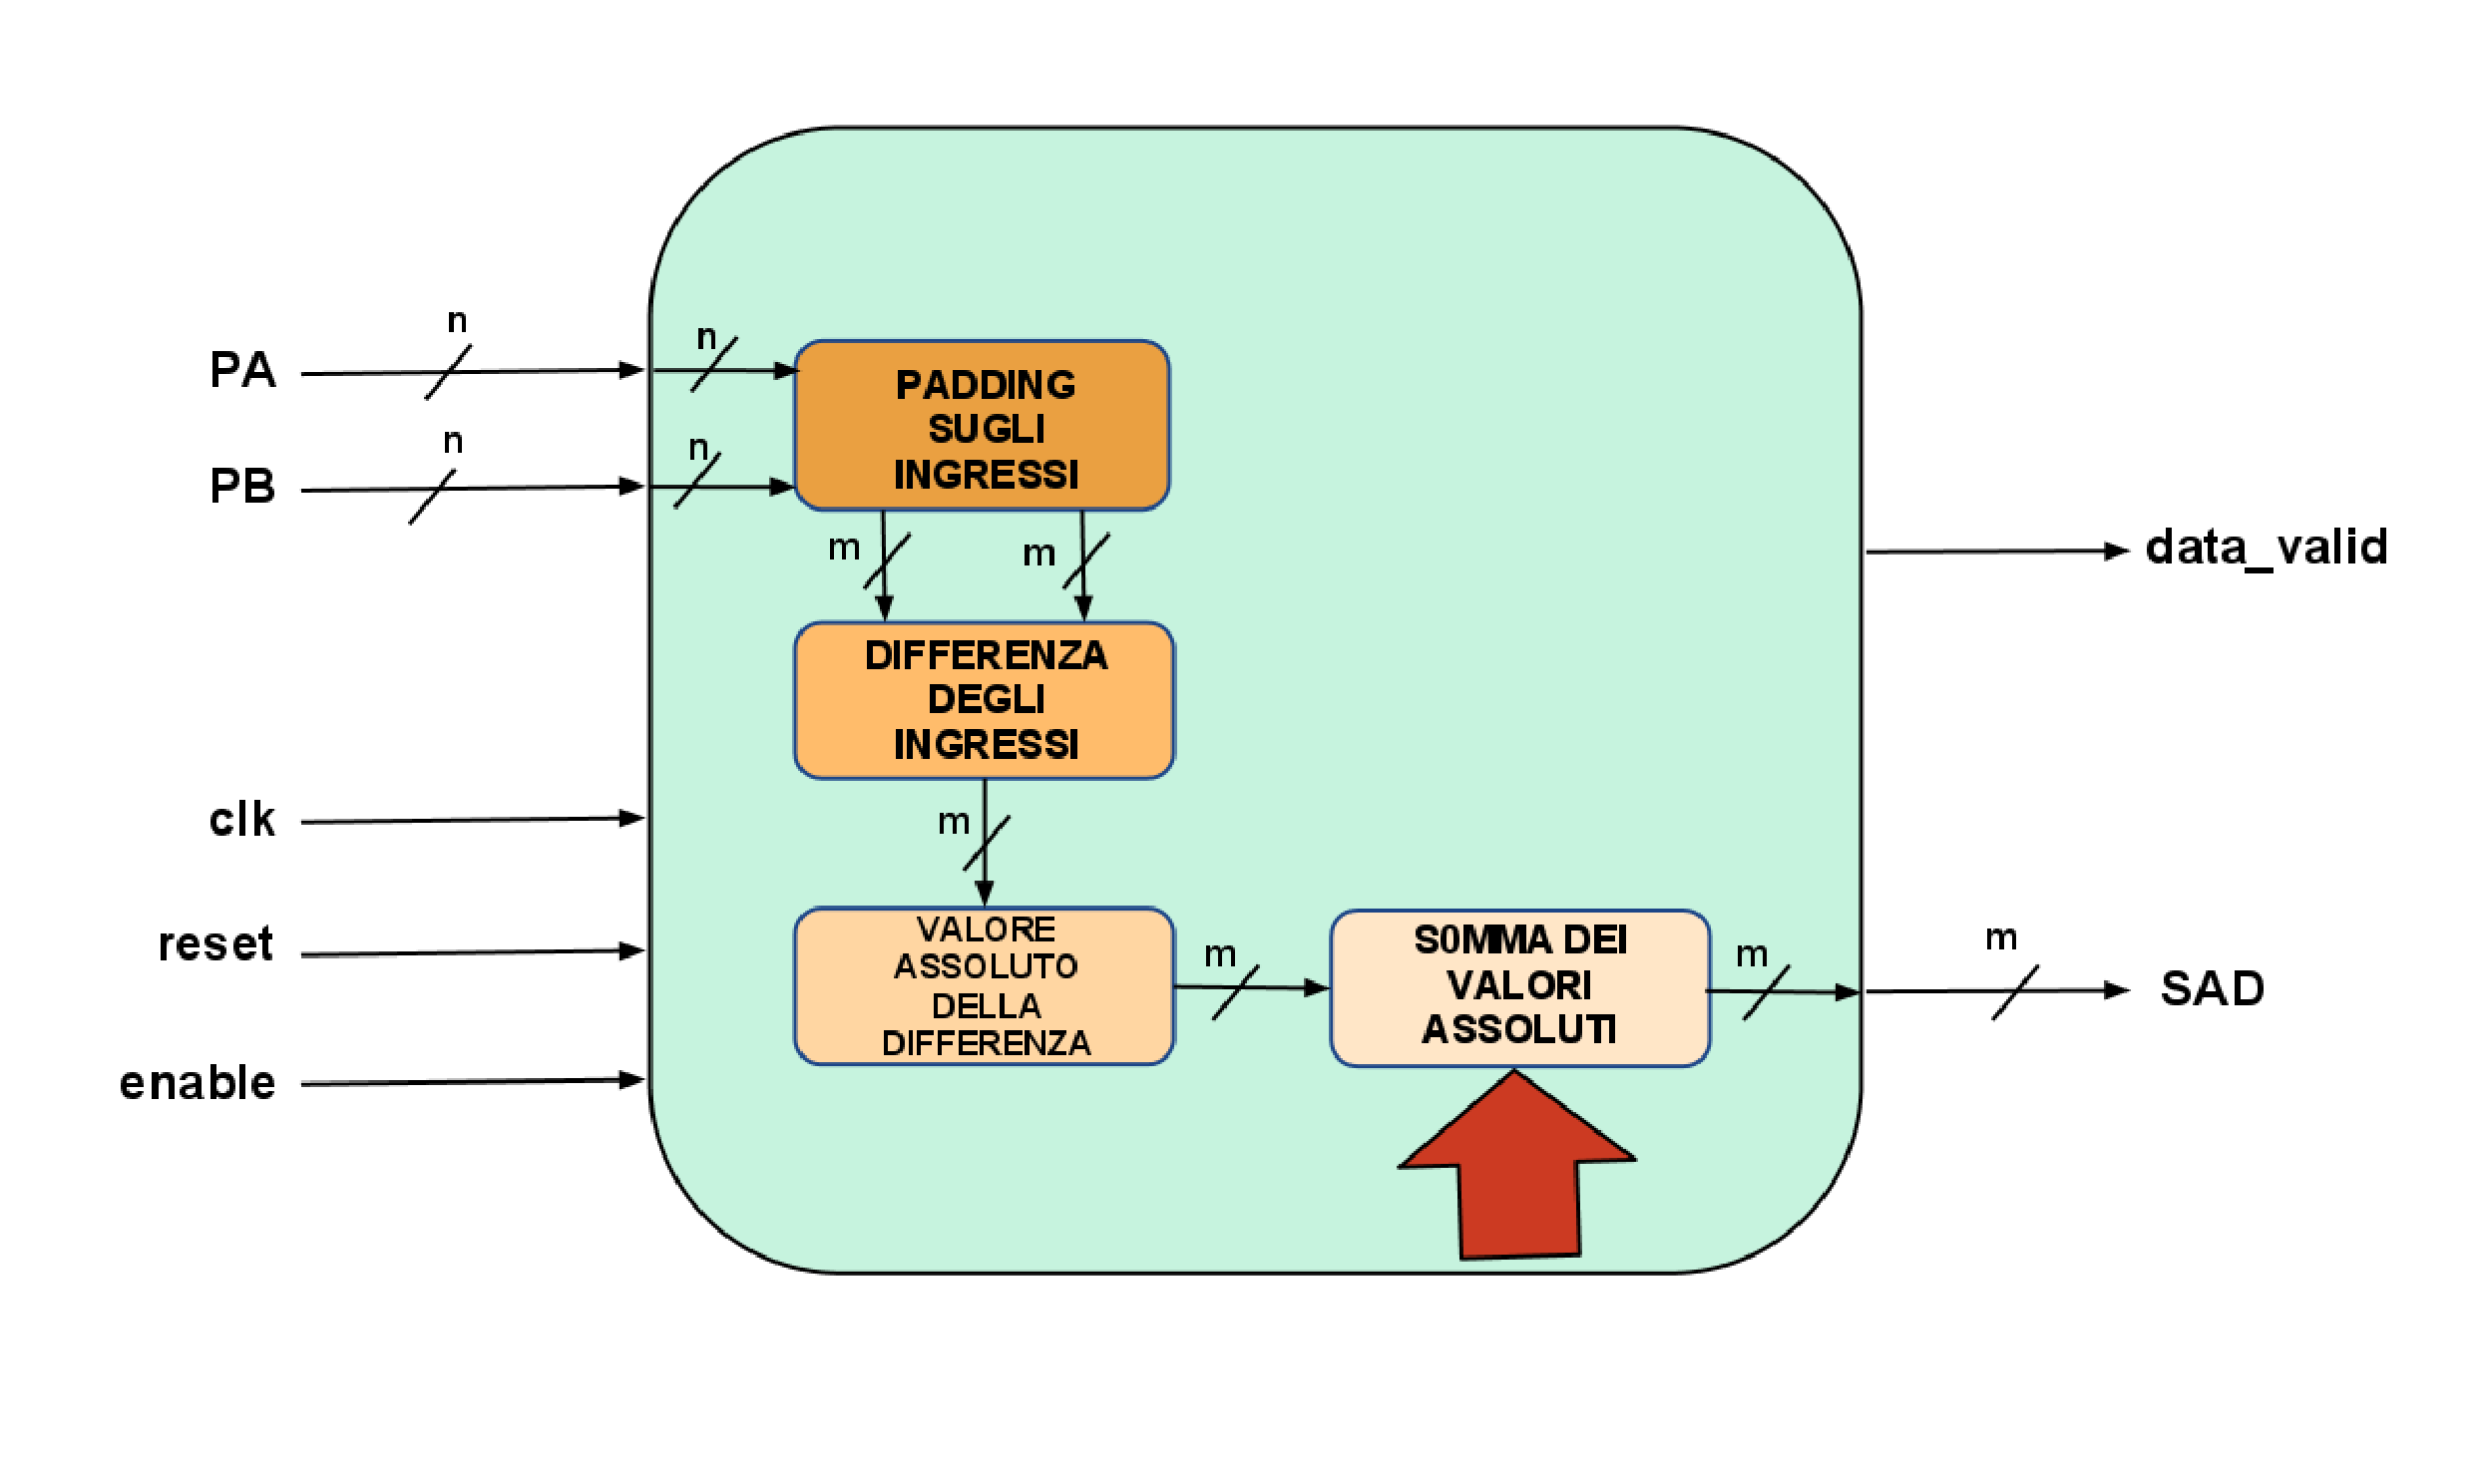
\includegraphics[scale=0.3]{images/somma.eps}
\caption{Modulo Somma}\label{fig:7}
\end{figure}
\newpage
\section{Testbench}
Per controllare il corretto funzionamento del circuito sono stati realizzati due \textit{testbench} (uno per il caso specifico e uno per il caso generale) settando gli ingressi come segue: \textit{PA} = 5 e \textit{PB} = 10. Come si vede dai grafici riportati in basso (relativi al caso specifico) tutti i segnali funzionano in maniera corretta e il calcolo della \textit{SAD} a conclusione delle operazioni corrisponde a quello atteso.
\begin{figure}[h!]
\centering
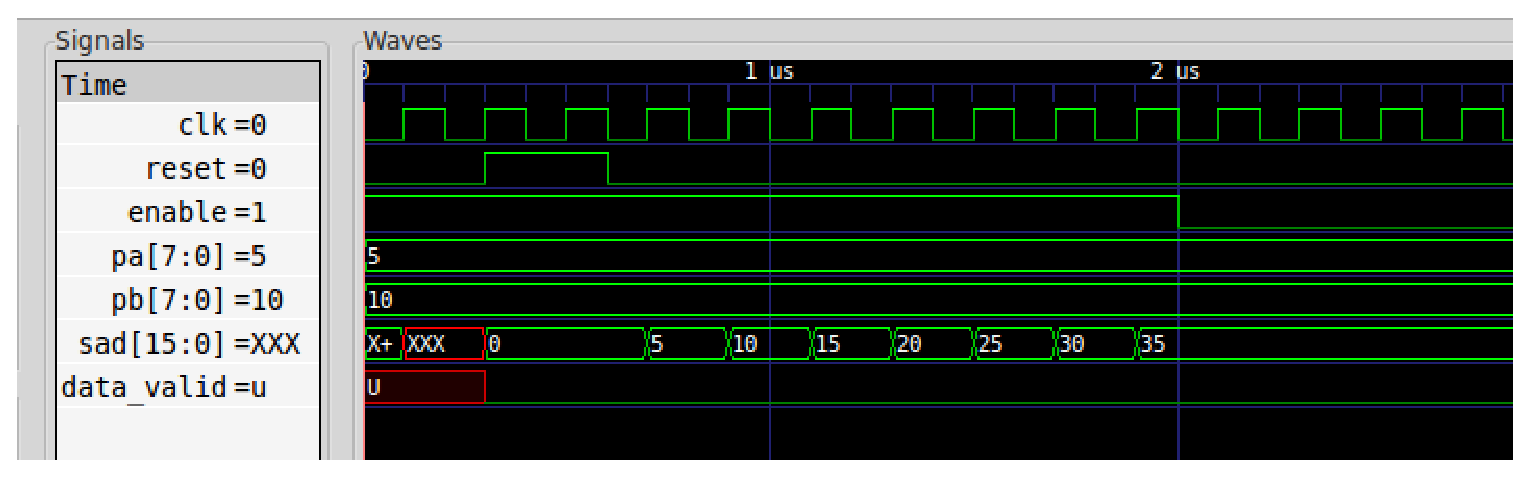
\includegraphics[scale=0.45]{images/tb1.eps}
\caption{Testbench - Parte iniziale}\label{fig:8}
\end{figure}
\begin{figure}[h!]
\centering
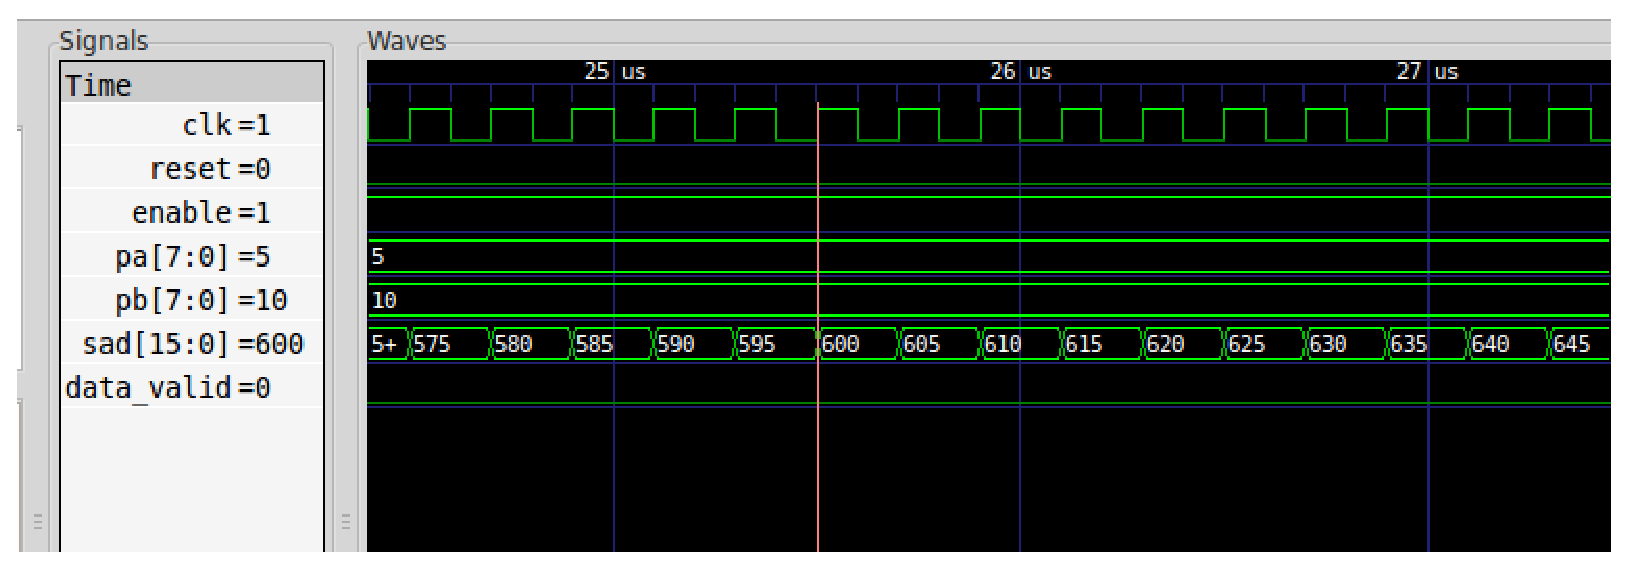
\includegraphics[scale=0.4]{images/tb2.eps}
\caption{Testbench - Parte centrale}\label{fig:9}
\end{figure}
\begin{figure}[h!]
\centering
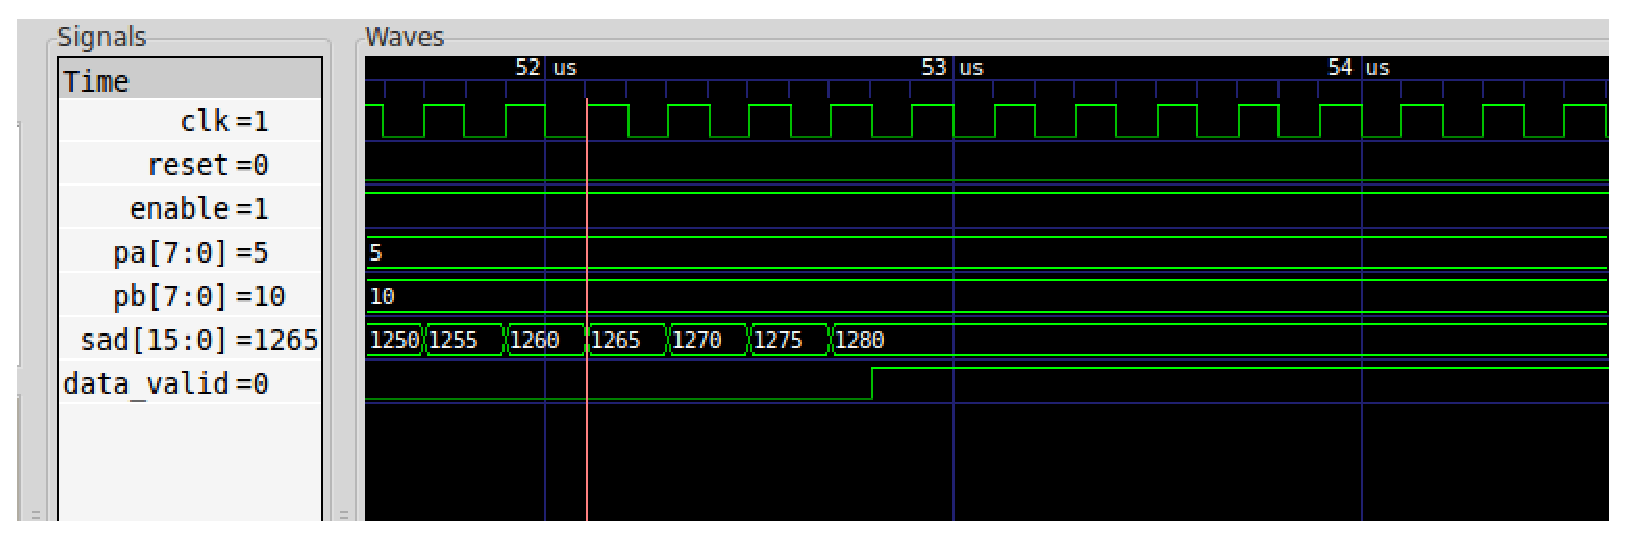
\includegraphics[scale=0.45]{images/tb3.eps}
\caption{Testbench - Parte finale}\label{fig:10}
\end{figure}
\newpage
\section{Istruzioni di compilazione ed esecuzione}
Il progetto è stato realizzato in ambiente GNU/Linux utilizzando i tool GHDL (per la compilazione e la creazione degli eseguibili) e GTKWave (per la visualizzazione delle temporizzazioni).\\
Per compilare l'applicazione posizionarsi nella directory \textit{/src} e digitare da shell:
\begin{itemize}
\item
\textit{make sad }- nel caso si voglia compilare il codice relativo al caso specifico;
\item
\textit{make test} - nel caso si voglia compilare il codice relativo al test del caso specifico;
\item
\textit{make sad\_n }- nel caso si voglia compilare il codice relativo al caso generale;
\item
\textit{make test\_n} - nel caso si voglia compilare il codice relativo al test del caso generale;
\item
\textit{make} - nel caso si vogliano compilare tutte le parti di codice sopra elencate. 
\end{itemize}
Per visualizzare il testbench posizionarsi nella directory \textit{/testbench} e digitare da shell:
\begin{itemize}
\item 
\textit{gtkwave sad.vcd} - nel caso si voglia visualizzare la temporizzazione relativa al caso specifico;
\item
\textit{gtkwave sad\_n.vcd} - nel caso si voglia visualizzare la temporizzazione relativa al caso generale.
\end{itemize}
\end{document}